
\section{Vers une prise en compte plus générale de l'exposition}

Au cours de ma thèse, plusieurs questions ont pu être adressés et certaines réponses
apportées.  Cependant, le choix a été fait de se limiter principalement sur l'estimation
des sources de PO à travers le modèle PMF. Bien qu'apportant des résultats éclairant sur
la dynamique des PO, plusieurs aspects ont été volontairement écartés de ces études.

Premièrement, l'utilisation de modèle site-récepteur limite nécessairement la couverture
spatiale et temporelle à quelques sites d'études et années de mesures. Or la
généralisation d'une estimation des mesures de PO à tous points spatio-temporel est
souhaitable lorsque l'on s'intéresse à coupler dans une même étude mesures
épidémiologiques et qualité de l'air.

Deuxièmement, la méthode utiliser pour estimer un PO par sources de PM présente un
développement mathématique linéaire. Or, on sait que le PO ne réagit pas de manière
linéaire à la masse des composés chimiques. Si ce modèle présente une première
approximation, il est, par construction, limité et biaisé.  Il existe cependant des
modèles d'inversion non-linéaire qui permettraient la prise en compte des interactions
entre sources et composés chimiques dans l'estimation des sources de PO.

Finalement, jusqu'à présent seuls des prélèvements en air extérieur ont été considérés. Or
nous passons la plus grande partie de notre temps en espace clos intérieur (maison,
appartement, bureau, voiture, etc.).  La représentativité des mesures en air extérieur
comme référence de l'exposition de la population n'est donc peut-être suffisante.

\section{Spatialisation du PO}

\subsection{Estimation du PO à partir des PM}

Dans cette thèse, deux synthèses nationnales grande échelle ont été faite : 1) estimation
des contributions des sources de PM à la masse \autocite{weberComparison2019}
(chapitre~\ref{cha:estimation_des_sources_de_PO}) et 2) attribution du PO intrinsèque à
chacune des sources de PM majoritairement présentes \autocite{weberSourceinprep.}
(chapitre~\ref{cha:estimation_des_sources_de_PO}).

Ainsi, et en première approximation, il est possible d'estimer la contribution moyenne
relative mensuelle des différentes sources à la masse totale des PM. Puis, connaissant le
PO intrinsèque (i.e. par microgramme de PM) de chacune de ces sources, une simple
multiplication permet une estimation approximative du PO.  La conséquence est que pour
chaque valeur de concentration de \PMdix{} il est possible d'estimer, au premier ordre,
une valeur de PO associée.

Bien évidemment, cette méthode possède trois limitations fortes : 
\begin{itemize}
    \item Les contributions relatives des sources sont moyennées mensuellement d'après un
        ensemble de 15 sites de mesures, de typologie plutôt urbaine, et donc non
        nécessairement représentative de l'ensemble des situations possibles ;
    \item Le PO intrinsèque de chacune de ces sources présente en réalité une variabilité
        plus ou moins importante, et une fois de plus estimés à partir d'un ensemble de
        site de typologie plutôt urbaine ;
    \item Il n'est pas pris en compte la spécificité du site en question ni la possible
        évolution du PO intrinsèque des sources liés à possible une évolution du profile
        chimique (renouvellement de parc automobile, etc.).
\end{itemize}

Elle présente néanmoins l'avantage de pouvoir estimer pour n'importe quel site possédant
une concentration massique des \PMdix{} une mesure de \POAAv{} et \PODTTv. Il est
également possible d'utiliser ce procédé en post-traitement d'un modèle déterministe de
prévision de concentration de \PMdix.

Aussi, au fur et à mesure que de nouvelle étude se feront, il est tout à fait possible de
raffiner cette technique en ne sélectionnant que des sites de même typologie ou
environnement (rurale, vallée alpine, trafic, etc.) aussi bien pour la partie d'estimation
de la contribution des sources aux \PMdix{} que pour la partie attribution d'un PO
intrinsèque par source.

Afin de tester la faisabilité de cette méthode d'estimation au premier ordre du PO, le
site de Grenoble les Frènes a été choisi car bénéficie d'une série de mesure longue durée
du PO. Cette méthode est aussi rendu disponible grâce au développement du module python
\href{https://gricad-gitlab.univ-grenoble-alpes.fr/pmall/pyopestimator}{pyOPestimator},
disponible sur PyPi\footnote{\url{https://pypi.org/project/pyOPestimator/}} et sur la
forge de l'université de
grenoble\footnote{\url{https://gricad-gitlab.univ-grenoble-alpes.fr/pmall/pyopestimator}}.
Il est également possible d'utiliser directement
\url{http://getopstandop.u-ga.fr/estimate}, permettant d'estimer directement en ligne le
\POAAv{} et \PODTTv{} de n'importe quelle série de mesure concentration de \PMdix.

Les \POAAv{} et \PODTTv{} mesurés et estimés par cette méthode sont présentés
figure~\ref{fig:OPGRE-fr-estimated}.  Les cycles saisonnier sont bien retrouvés et les
amplitudes respectées. Cependant et comme attendu, certains évènements peu fréquent sont
mal estimés. Au final, une corrélation (Pearson) respective de 0.75 et 0.79 pour le
\POAAv{} et \PODTTv{} est obtenu en prenant en compte les 769 échantillons où les PO ont
été mesurés (voir figure~\ref{fig:OPGRE-fr-estimated_scatter}).  Considérant les grandes
approximations faites par cette méthode, ce résultat présente des performance étonnante !

\begin{figure}[ht]
    \centering
    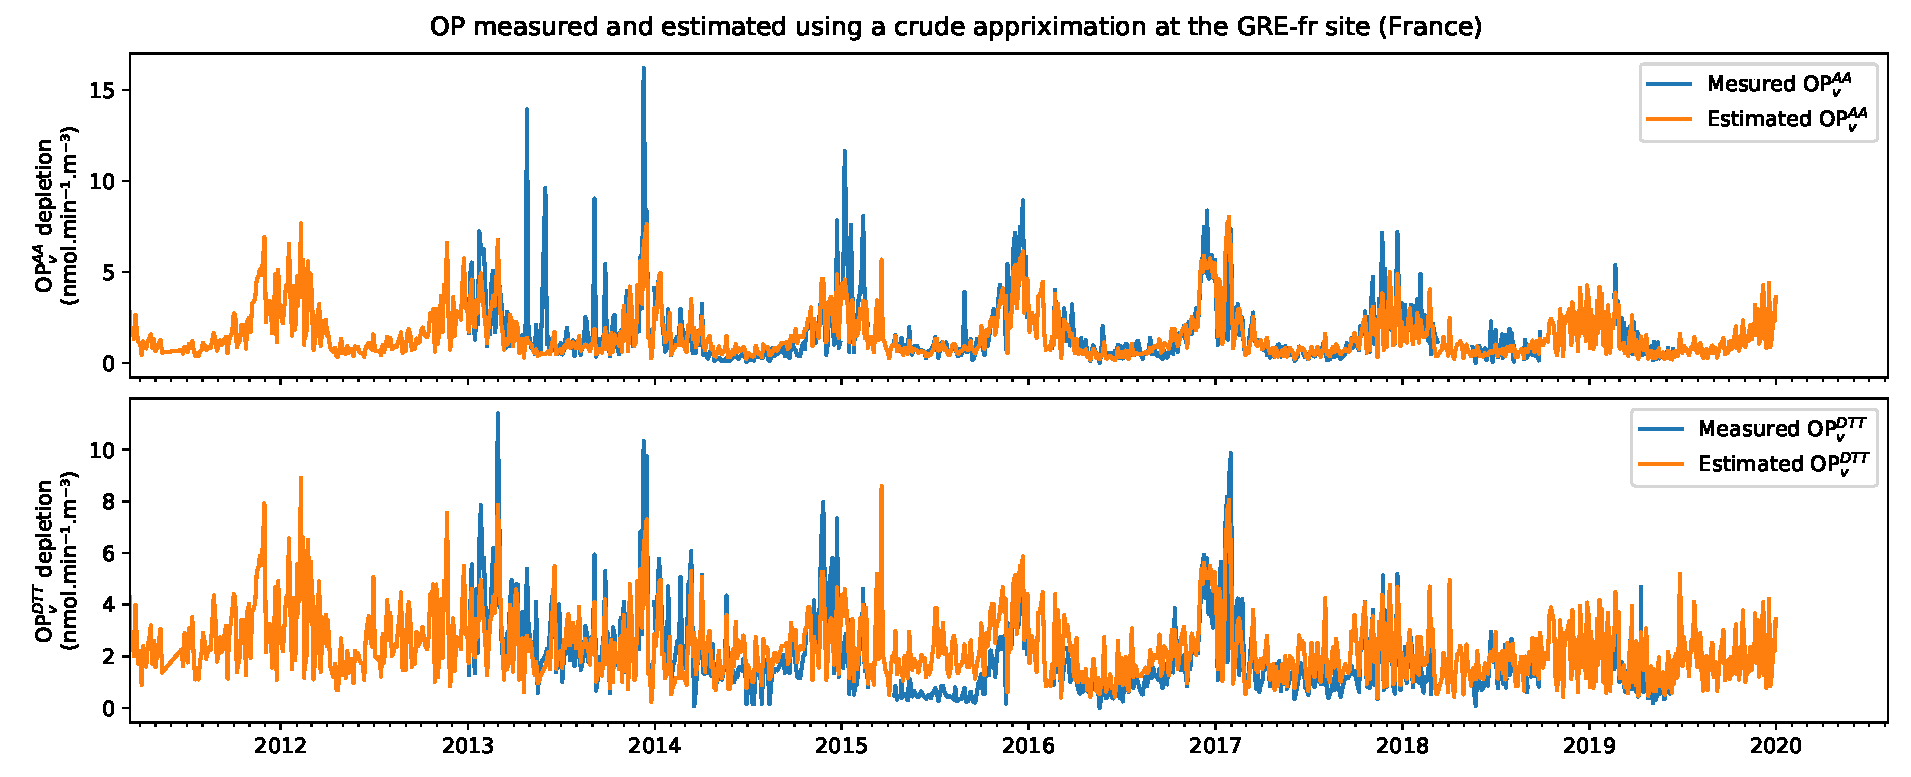
\includegraphics[width=1.0\textwidth]{figures/chapter05/OPGRE-fr_estimated.pdf}
    \caption{\POAAv{} (haut) et \PODTTv{} (bas) estimés en orange et mesurés en bleu sur le site de GRE-fr depuis 2011.}
    \label{fig:OPGRE-fr-estimated}
\end{figure}
 
\begin{figure}[ht]
    \centering
    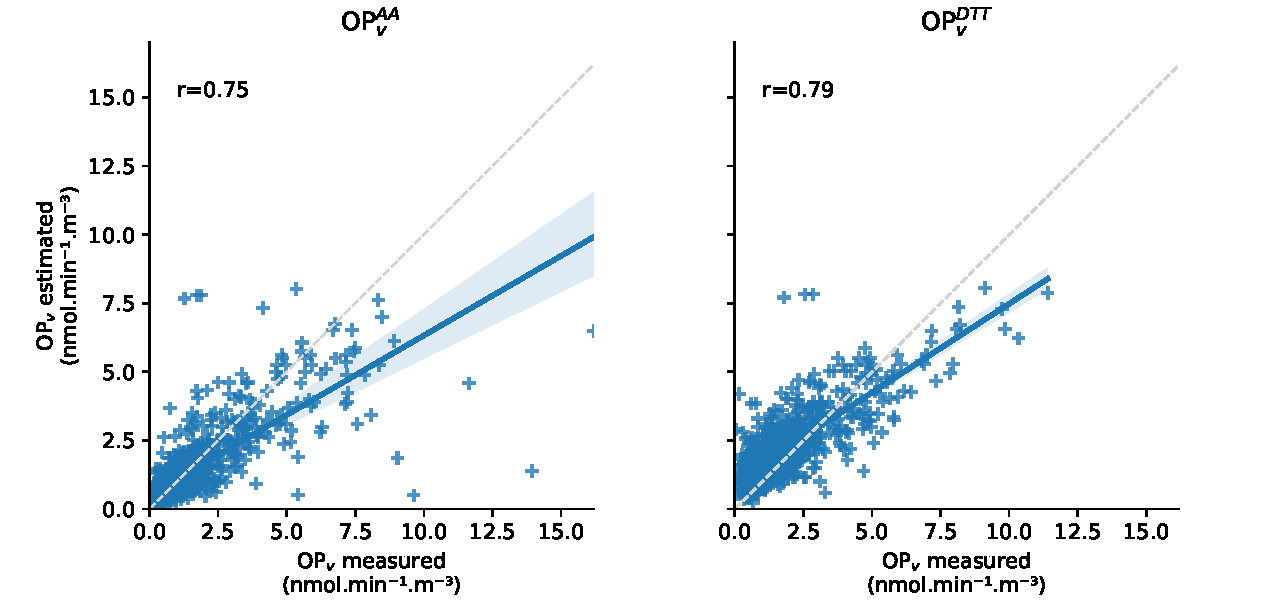
\includegraphics[width=0.8\textwidth]{figures/chapter05/OPGRE-fr_estimated_scatter.pdf}
    \caption{\POAAv{} et \PODTTv{} estimés et mesurés sur le site de GRE-fr depuis 2012.}
    \label{fig:OPGRE-fr-estimated_scatter}
\end{figure}


Il est donc possible d'estimer en premier ordre la contribution des sources majoriatire de
PM aux PO, et ce en prennant en compte l'intégralité des mesure annuelle disponible. La
prise en compte de toutes ces mesures nous affranchi du biais de sélection présent dû
fait de la fréquence d'échantillonage et d'annalyse sur filtre. Les contributions des
sources de PO d'après les mesures journalières d'Atmo AURA sur la station de GRE-fr sont
présentées figure~\ref{fig:OPGRE-fr_source_estimated} et détaillées dans le
tableau~\ref{tab:OPGRE-fr_source_estimated}.

Du fait de l'importance du PO intrinsèque de la source combustion de biomasse
(\textit{Biomass burning} dans le graphique), sa contribution moyenne annuelle est
également importante, notamment pour le \POAAv.  En revanche, puisque l'ont dispose de
l'ensemble des jours de mesures et que cette source présente une dynamique très
saisonnière, l'écart entre contribution moyenne et médiane est très important.
En revanche, conformément aux PO intrinsèque élevés de la source trafic primaire
(\textit{Road traffic} dans le graphique) et sa contribution relativement homogène tout au
long de l'année, cette source est la première contributrice au \PODTTv, aussi bien en
moyenne qu'en médiane.

Si elle n'apprend rien de bien nouveau, cette méthode d'estimation certes grossière,
permet la prise en compte d'un très grand nombre de jours d'observation et met d'autant
mieux en lumière la différence entre contribution moyenne et contribution médiane des
sources de \PMdix{} aux PO.

Enfin, il est possible de propager la variabilité aussi bien de la contribution mensuelle
moyenne de chacune de source que de leur PO intrinsèque dans cette methode. Ce travail n'a
pas encore été entammé, mais nous disposons de l'ensemble des informations nécessaire pour
cela.

En définitive, puisqu'il est raisonable d'estimer le PO des \PMdix{} par cette technique,
il parait envisageable d'établir une cartographie du PO à partir soit des mesures satellites
de concentration de \PMdix, soit des sorties de modèle CTM.

\begin{figure}[ht]
    \centering
    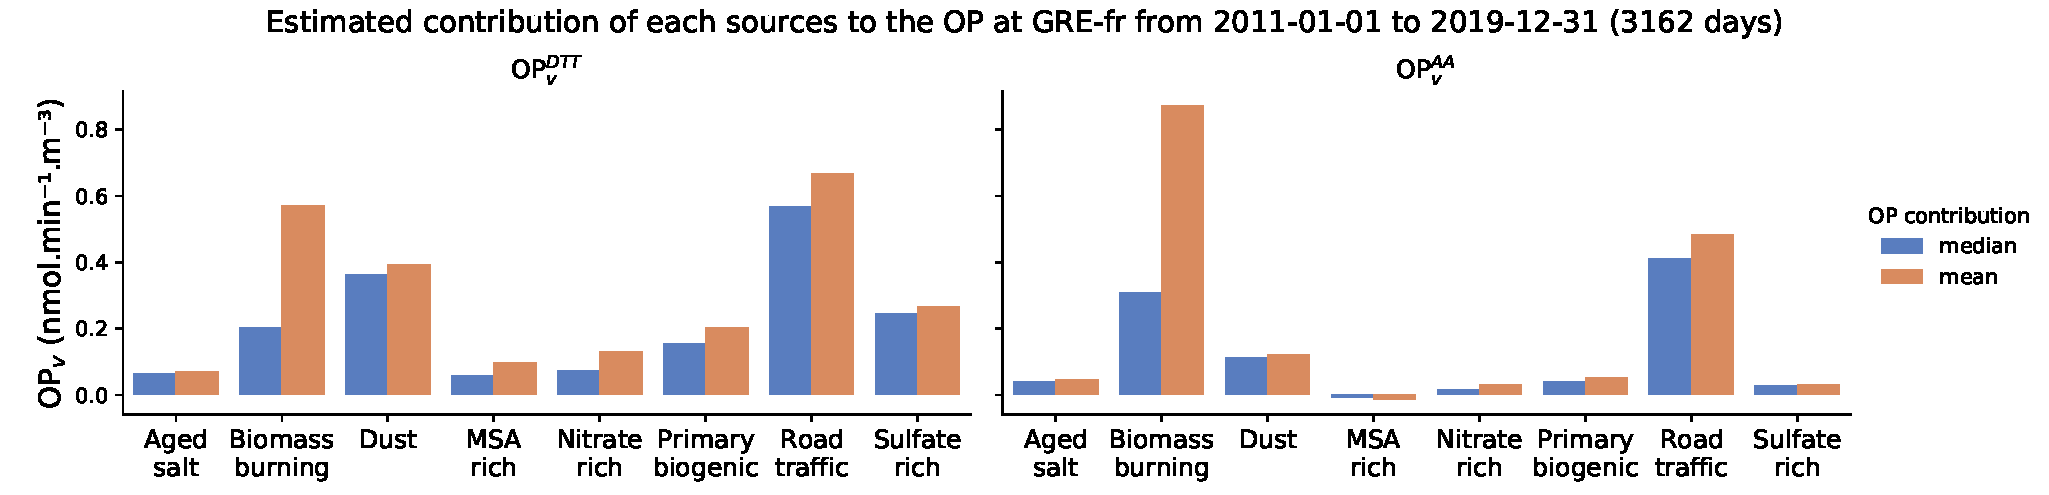
\includegraphics[width=1.0\linewidth]{figures/chapter05/OPGRE-fr_source_estimated.pdf}
    \caption{Contributions estimées moyennes et médianes des sources de \PMdix{} aux
        \PODTTv{} et \POAAv{} sur le site de Grenoble Les frènes entre 2011 et 2019.}%
    \label{fig:OPGRE-fr_source_estimated}
\end{figure}

\begin{table}[ht]
    \centering
    \footnotesize
    \begin{tabular}{cp{1cm}p{1.3cm}p{1.3cm}p{1.3cm}p{1.3cm}p{1.3cm}p{1.3cm}p{1.3cm}p{1.3cm}p{1.3cm}}
        \toprule
        & & \multicolumn{8}{c}{Estimated source contribution to OP in \si{\opv}}\\

                       &      & Aged salt & Biomass burning & Dust  & MSA rich & Nitrate rich & Primary biogenic & Road traffic & Sulfate rich\\\midrule

\multirow{6}{*}{AAv}   & mean & 0.045 & 0.871 & 0.121 & -0.014 & 0.030 & 0.051 & 0.482 & 0.031\\
                       & std  & 0.023 & 1.178 & 0.066 & 0.014  & 0.032 & 0.038 & 0.285 & 0.017\\
                       & min  & 0.002 & 0.008 & 0.005 & -0.114 & 0.001 & 0.001 & 0.041 & 0.001\\
                       & 25\% & 0.028 & 0.066 & 0.074 & -0.020 & 0.007 & 0.021 & 0.275 & 0.019\\
                       & 50\% & 0.041 & 0.308 & 0.111 & -0.008 & 0.016 & 0.038 & 0.409 & 0.028\\
                       & 75\% & 0.058 & 1.265 & 0.158 & -0.004 & 0.042 & 0.072 & 0.626 & 0.041\\
                       & max  & 0.167 & 6.347 & 0.502 & -0.000 & 0.259 & 0.235 & 1.867 & 0.138\\
                          \midrule
 \multirow{6}{*}{DTTv} & mean & 0.070 & 0.571 & 0.392 & 0.096 & 0.131 & 0.202 & 0.668 & 0.266\\
                       & std  & 0.036 & 0.772 & 0.214 & 0.096 & 0.142 & 0.153 & 0.395 & 0.145\\
                       & min  & 0.003 & 0.005 & 0.016 & 0.001 & 0.004 & 0.006 & 0.057 & 0.013\\
                       & 25\% & 0.043 & 0.043 & 0.239 & 0.027 & 0.033 & 0.084 & 0.382 & 0.162\\
                       & 50\% & 0.064 & 0.202 & 0.361 & 0.058 & 0.073 & 0.154 & 0.568 & 0.245\\
                       & 75\% & 0.090 & 0.829 & 0.510 & 0.140 & 0.184 & 0.286 & 0.868 & 0.348\\
                       & max  & 0.261 & 4.162 & 1.623 & 0.772 & 1.129
                       & 0.937 & 2.587 & 1.170\\
                          \bottomrule
    \end{tabular}
    \caption{Contributions estimées des sources de PM aux \POAAv{} et \PODTTv{} pour
    Grenoble Les Frènes entre 2011 et 2019 (n=3162 jours)}
    \label{tab:OPGRE-fr_source_estimated}
\end{table}


\subsection{Prévision déterministe du PO (modélisation CTM)}

Si la partie précédente présentait une méthode approximative de prévision du PO à partir
du calcul de la masse des \PMdix{} estimée par les CTM, il est certainement cependant
préférable d'inclure directement la variable ``potentiel oxydant'' dans ces modèles.

Cependant, le ``PO'' n'étant pas une espèce chimique évoluant et réagissant, son
estimation ne peut se faire que a posteriori et à partir soit du PO intrinsèque de chacune
des espèces chimiques, soit en estimant la contribution des sources à la masse de \PMdix
Mais les mêmes limitations que pour l'inversion par espèces chimiques se retrouve. Il faut donc
réussir à estimer les sources de \PMdix{} dans les modèles CTM.

Ensuite, deux solutions sont envisageables:
\begin{enumerate}
    \item estimer un PO intrinsèque par source d'émission des CTM en utilisant le même
        procédé que celui développée durant cette thèse en utilisant les mesures de PO à
        différentes stations;
    \item établir une équivalence entre source CTM et facteur PMF, puis appliquer les
        PO intrinsèque des facteurs PMF aux sources estimées par CTM.
\end{enumerate}

La première solutions permettrait le prise en compte d'un nombre de source beaucoup plus
grand que celles retenues dans les PMF (émission portuaire, différent type de résidentiel
ou trafic, feu de forêt, etc) puisque les sources des CTM sont fondées sur les SNAP, qui
sont très nombreux.
En revanche, cette solution, dans son implémentation actuelle à travers le ``source
labelling'', ne prend en compte uniquement les sources primaires. Par exemple, la
condensation des NOx du trafic routier et de l'ammoniac de l'agriculture forme du
nitrate-d'ammonium et est attribué selon une moyenne pondérée à la source trafic et
agricole. Il y a donc une perte d'information entre source primaire et secondaire.

La deuxième solution nécessite une comparaison des émissions chimique considérés dans
chacun des SNAP utilisés avec les profils chimiques des facteurs PMF. S'il est possible
d'établir un rapprochement entre ces 2 nomenclatures, il sera possible d'estimer le PO
apporté par ces sources.

Dans les 2 cas, le développement de la technique de ``source-labelling'' et la base de
donnée unique d'attribution des sources en site récepteur appelle à une étude de
sensibilité des prédiction des CTM. Notamment, LOTOS-EUROS\footnote{LOTOS-EUROS:
    \url{https://lotos-euros.tno.nl/}} (abbrégé LE) développé au TNO (\textit{Netherlands Organisation for
Applied Scientific Research}) a récemment rendu disponible à travers TOPAS\footnote{TOPAS:
TNO Operational Pollution Apportionment Service (\url{https://topas.tno.nl/})}. Cette
avancée est rendu possible par l'implémentation de \cite{kranenburgSource2013} dans
LOTOS-EUROS v2 \autocite{mandersCurriculum2017}.

Une collaboration entre l'IGE et le TNO a donc été engagée afin de confronter les
prédictions de LE aux sorties PMF. Aussi, dans lors de mon séjour en 2018, nous
avons pu apporté une preuve de concept de la faisabilité de la prédiction du PO par
LE pour 2 sources chimiquement proches entre LE et les PMF.
La figure~\ref{fig:OPmap} présente pour 10 février 2017 à 11:30 la contribution du
transport routier et de la combustion résidentielle à la masse et au \PODTTv{} pour
l'ensemble de l'Europe.

Ce travail, très préliminaire, se poursuivra après ma thèse dans le cadre de cette
collaboration entre l'IGE et le TNO.

\begin{figure}[ht]
    \centering
    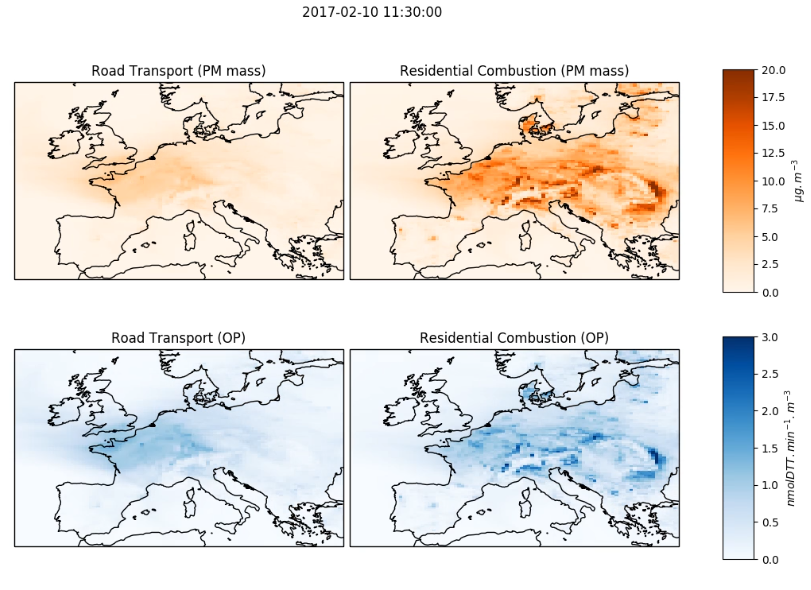
\includegraphics[width=0.8\linewidth]{figures/chapter05/OPmap.png}
    \caption{Preuve de concept de la modélisation grande échelle du potentiel oxydant,
    utilisant le \PODTT{} intrinsèque du trafic routier et de la combustion de biomasse
estimée par \cite{weberSourceinprep.} appliqué aux prévisions de LOTOS-EUROS.}%
    \label{fig:OPmap}
\end{figure}

Cette preuve de concept en 2018 a aiguisé la curiosité des chercheurs et développeurs
d'un autre modèle de chimie transport: Chimère. Chimère a donc maintenant implémenté la
même technique de ``source-labelling'' et un travail identique à celui entammé avec le
TNO et LE est en cours avec le LISA et Chimère. Notamment, de février à juillet 2020, le
stage de M2 de Matthieu Vida portait sur cette thématique, qu'il va poursuivre en thèse à
la rentrée universitaire 2020.

Parallélement, \cite{daellenbachSourcessubmitted} ont conduit une étude similaire à celle
de \cite{weberSourceinprep.}, mais n'incluant que 109 mesures composites de potentiel
oxydant sur 6 sites de prélèvement en Suisse. Dans cette étude, à laquelle j'ai pris
part, le couplage entre PO intrinsèque et sources déterminée par le CTM CAMx est proposé.
Les résultats obtenus, présentée figure~\ref{fig:map_kaspard}, montre une fois de plus
l'importance de la combustion de biomasse mais aussi de la source trafic routière dans
les zones densément peuplées. En estimant l'exposition des populations comme la masse de
\PMdix{} ou la quantité de \POv{} inhalé, cette étude montre une fois de plus une
redistribution complète de l'importance des sources entre concentration massique et
potentiels oxydants. Encore une fois, l'importance du trafic routier s'accroit
considérablement et l'aérosol inorganique, pourtant dominant en terme de masse, n'a plus
qu'une influence minime sur l'exposition aux \POv.

Le même type d'étude, fondée sur une représentativité spatiale et temporelle plus
importante à l'échelle européenne est envisagée dans le cadre de mon
post-doctorat\footnote{sous réserve de validation de cette thèse bien entendu}.

\begin{figure}[ht]
    \centering
    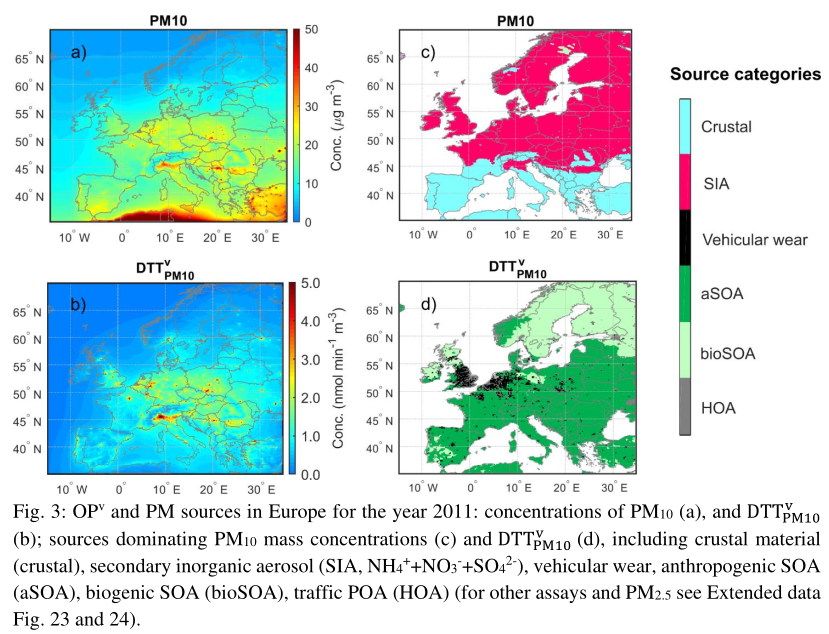
\includegraphics[width=0.8\linewidth]{figures/chapter05/map_kaspard.png}
    \caption{Estimation européenne du \PODTTv{} et des sources associées par
    \cite{daellenbachSourcessubmitted}.}%
    \label{fig:figures/chapter05/map_kaspard}
\end{figure}

\section{Non linéarité avec Réseaux de neurone}

\cite{borlazaUrbaninprep.}

\begin{figure}[ht]
    \centering
    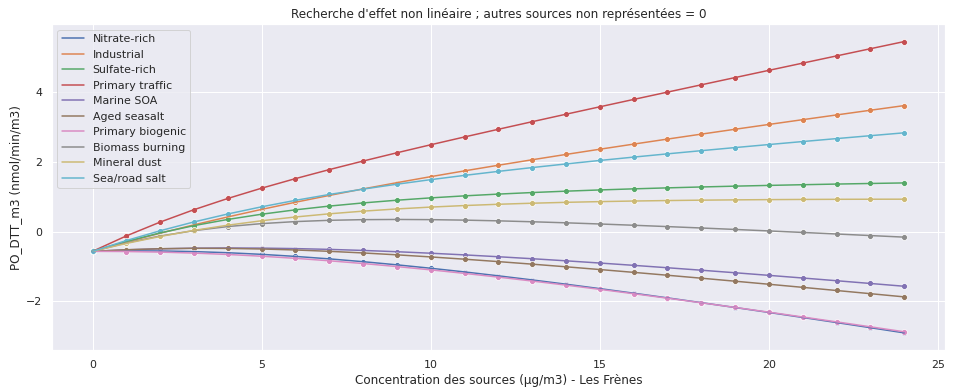
\includegraphics[width=0.8\linewidth]{figures/chapter05/10sourcesLinearite.PNG}
    \caption{Effet non linéaire de l'augmentation de la concentration d'une source
        d'émission sur le \PODTTv{} d'après le réseau de neurone entrainé sur Grenoble Les
    frènes lors du stage de M2 de Jean-Baptiste Fiches.}%
    \label{fig:figures/chapter05/10sourcesLinearite}
\end{figure}

\section{Exposition et épidémiologie}
\subsection{Mesure indoor et personnelle}
\subsection{Étude épidémio}

